\section{Heat Content in Annulus}

Since the heat (diffusion) equation defined in an annulus possesses explicit
solutions, the analytical expressions of heat content, derived by the
integration over the whole domain, are accessible. In this section,
the preliminary step is to solve the initial-boundary value problem
(IBVP) defined in the annulus. The numerical methods will then be used
to approximate that heat content, which helps validate the research
methodology in the next chapter.

\subsection{Analytical Results}

The heat equation Eq.$(2.1)$ defined in the polar coordinate system
describes the heat distribution varying in time and $\Omega$, as shown
in Figure $2.1$. The solution $u(r, \theta, t)$ implies the
temperature over spatial positions and time. In this subsection, the
primary purpose is to calculate the total amount of heat contained in
$\Omega$, heated at some nonzero temperature, in which $\partial
\Omega_{1}$ is cooled to the zero temperature and $\partial
\Omega_{2}$ is perfectly insulated.

\begin{equation}
  u_t = D \big(u_{rr} + \frac{1}{r} u_r + \frac{1}{r^2} u_{\theta\theta}\big)  
\end{equation}

\begin{equation}
  u = 0 \; \; \; on \; \partial \Omega_1
\end{equation}

\begin{equation}
  u' = 0 \; \; \; on \; \partial \Omega_2
\end{equation}


\begin{equation}
  u(r, \theta, 0) = \frac{1}{|\Omega|}
\end{equation}


where $D$ is the diffusion coeffiecnt, $r$ is radial coordinate,
$\theta$ is the angular coordinate, and $t$ is the time.

$u(r, \theta, t)$ is a probability density function, which gives the
value of heat particles at $(r, \theta)$ at time $t$. Eq.$(2.2)$ and
Eq.$(2.3)$ indicate the Dirichlet boundary condition on $\partial
\Omega_1$ and the Neumann boundary condition on $\partial \Omega_2$,
respectively. In other words, the heat particles will be absorbed when
they encounter with $\partial \Omega_1$ and be reflecting when they
reach $\partial \Omega_2$. Eq.$(2.4)$ states that the heat particles
distribute uniformly over the whole domain at time $t=0$, where
$|\Omega|$ equals the total area of the annulus.


\clearpage


\begin{figure}[h!]
  \begin{center}
    
\includegraphics[width=0.5\linewidth]{annulus.png}
    \caption{Assume the annulus $\Omega$ is a homogeneous and
      isotropic medium and has the inner boundary $\partial \Omega_1$
      with radius $a$ and outer boundary $\partial \Omega_2$ with
      radius $b$.}
  \end{center}
\end{figure}



\subsubsection{Solving Heat (Diffusion) Equation}

Before solving the heat equation, it is convenient and efficient to
generate dimensionless variables by dimensional analysis. The benefit
of dimensional analysis is that many physical parameters can be
combined into a smaller number of unitless variables, which do not
depend on the unit of the measurements and can also describe the
phenomenon or system of interestt \cite{barenblatt1996scaling}.


Define $\mu = b/a$ as the dimensionless radius ratio, $\tau =
\frac{Dt}{a^2}$ as the dimensionless time, and $\hat r = \frac{r}{a}$
as the unitless radius. Substitute the dimensionless variables and
rewrite Eq.$(2.1)$ as

\begin{equation}
  u_\tau = \big(u_{\hat r \hat r} + \frac{1}{\hat r} u_{\hat r} + \frac{1}{\hat r ^2} u_{\theta\theta}\big)
\end{equation}

With the uniform initial condition,
$$u\big(\hat r, \theta, 0\big) = \frac{1}{|\Omega|}$$

With the boundary conditions
$$u\big(1, \theta, \tau\big) = 0$$
$$u'\big(\mu, \theta, \tau \big) = 0$$

\clearpage

After implementing the separation of variables method
\cite{crank1979mathematics}, the solutions of Eq.$(2.5)$ are

\begin{equation}
  u\big(\hat r, \theta, \tau \big) = \sum_{n=1}^{\infty}
  \tilde{c_{0,n}} \bigg\{J_0\big(\sqrt{\lambda_{0,n}}\big)
  Y_0\big(\sqrt{\lambda_{0,n}} \hat r\big) -
  Y_0\big(\sqrt{\lambda_{0,n}}\big) J_0\big(\sqrt{\lambda_{0,n}} \hat
  r\big)\bigg\} e^{-\lambda_{0,n}\tau}
\end{equation}

where

$$\tilde{c_{0,n}} = \frac{1}{\big(\mu^2 - 1\big)}
\frac{1}{\bigg[\frac{J_0\big(\sqrt{\lambda_{0,n}}\big)}{J'_0\big(\mu
      \sqrt{\lambda_{0,n}}\big)}\bigg]^2 -1}$$


Eigenvalues $\lambda_{0, n}$ $(n \in \mathbb{N}_{+})$ is $n$th
positive root of the cross-product of Bessel functions
\cite{watson1995treatise}

\begin{equation}
  F_0(\lambda) = J_0(\sqrt{\lambda}) Y_0'(\sqrt{\lambda} \mu) -
  J_0'(\sqrt{\lambda} \mu) Y_0(\sqrt{\lambda})
\end{equation}



\subsubsection{Heat Content (Survival Probability)}

The amount of heat contained in $\Omega$ at the moment $\tau > 0$
defined as heat content $Q_{\Omega}(\tau)$, which is an alternative
terminology of survival probability in some mathematical literatures
\cite{birkhoff1954note} \cite{van1994heat}
\cite{gilkey1994heat}. Survival probability $S(\tau)$ is proportional
to $Q_{\Omega}(\tau)$ \cite{kalinay2011survival}, which gives the
probability of the particles remain diffusing in the domain $\Omega$
at time $\tau > 0$ \cite{aalen2008survival}. Survival probability can
be expressed by

\begin{equation}
  \begin{split}
    S(\tau) &= \int_{0}^{2\pi} d\theta \int_{1}^{\mu} \hat r d \hat r
    u(\hat r, \theta, \tau)\\ &= \sum_{n=1}^{\infty} \frac{4}{\mu^2 -
      1} \frac{1}{\lambda_{0,n}
      \bigg\{\bigg[\frac{J_0(\sqrt{\lambda_{0,n}})}{J'_0(\mu
          \sqrt{\lambda_{0,n}})}\bigg]^2 -1\bigg\}} e^{-\lambda_{0, n}
      \tau}
  \end{split}
\end{equation}

From Eq.$(2.8)$, we can find some basic properties of
$S(\tau)$. Firstly, when $\tau=0$, the survival probability is $1$
since all the particles are just generated over the whole domain and
not be absorbed by $\Omega_1$. Secondly, $S(\tau)$ is a convergent
series with multiexponential decay. Thirdly, $S(\tau)$ interconnects
the overall geometric characteristics of $\Omega$. For example, the
decay rate of $S(\tau)$ in a short time heavily depends on the
geometrical features of $\Omega_1$, as only the particles inserted
close to $\Omega_1$ have the high probabilities of being
absorbed. Finally, as the lone-time limit, $S(\tau)$ is represented by
the lowest eigenvalue $\lambda_{0, 1}$.

\subsubsection{Mean First-Passage Time}


The first passage phenomena play a fundamental role in stochastic
processes triggered by a first-passage event
\cite{van1992stochastic}. One of the essential first-passage-related
quantities is the first-passage probability, which is a probability of
diffusing particle or a random-walk hitting a specified site or a set
of sites at a specified time for the first time
\cite{redner2001guide}. All the first-passage characteristics can be
expressed in terms of first-passage probability itself. For example,
the survival probability at time $\tau$ calculated in the last
subsection has

\begin{equation}
  F(\tau) = - \frac{\partial S(\tau)}{\partial \tau}
\end{equation}

where $F(\tau)$ is the first-passage probability to the target
boundary at time $\tau$. By the definition, the $n$th moment of the
exit time \cite{redner2001guide} is

\begin{equation}
  \begin{split}
    \langle \tau^n \rangle &= \int_{0}^{\infty} \tau^n F(\tau) d\tau \\
    &= - \int_{0}^{\infty} \tau^n  \frac{\partial S(\tau)}{\partial \tau} d\tau \\
    &= -\tau^n S(\tau) |_{0}^{\infty} + n\int_{0}^{\infty} \tau^{n-1}S(\tau) d\tau
\end{split}
\end{equation}


Substitue $n=1$ in Eq.$(2.10)$, the mean-first passage time $\langle
\tau \rangle$, also called the average first-passage time, of a group
of particles implies an overall property of the system is

\begin{equation}
  \begin{split}
    \langle \tau \rangle &= \int_{0}^{\infty} \tau dS\\
    &=\sum_{n=1}^{\infty} \frac{4}{\mu^2 - 1}
    \frac{1}{\lambda^2_{0,n}\bigg\{\bigg[\frac{J_0(\sqrt{\lambda_{0,n}})}{J'_0(\mu\sqrt{\lambda_{0,n}})}\bigg]^2
      -1\bigg\}}
  \end{split}
\end{equation}



\newpage

\subsection{Numerical Analysis}

Numerical analysis is an area of mathematics and computer science that
creates, analyzes, and implements algorithms for approximating
numerical solutions to problems involving continuous variables
\cite{brezinski2012numerical}. For simplicity, a specific kind of
annulus is considered, which has the radius ratio $\mu=2$. 

The preliminary step of the evaluation of $S(\tau)$, a general
Dirichlet series, and $\langle \tau \rangle$ is to compute the
monotonically increasing $\lambda_{0,n}$ of Eq.$(2.7)$. The $n$th
positive zero $\lambda_{0,n}$, as $n \rightarrow \infty $, can be
bracketed in an interval $((n-1) \pi, (n+1) \pi)$
\cite{NIST:DLMF}. Bisection method \cite{2020SciPy-NMeth}, a
well-known and most reliable root finding method. It can be used to
close in on the root by successivly halving the interval until it
becomes sufficiently small.

\begin{figure}[h!]
  \centering
  \subfloat[]{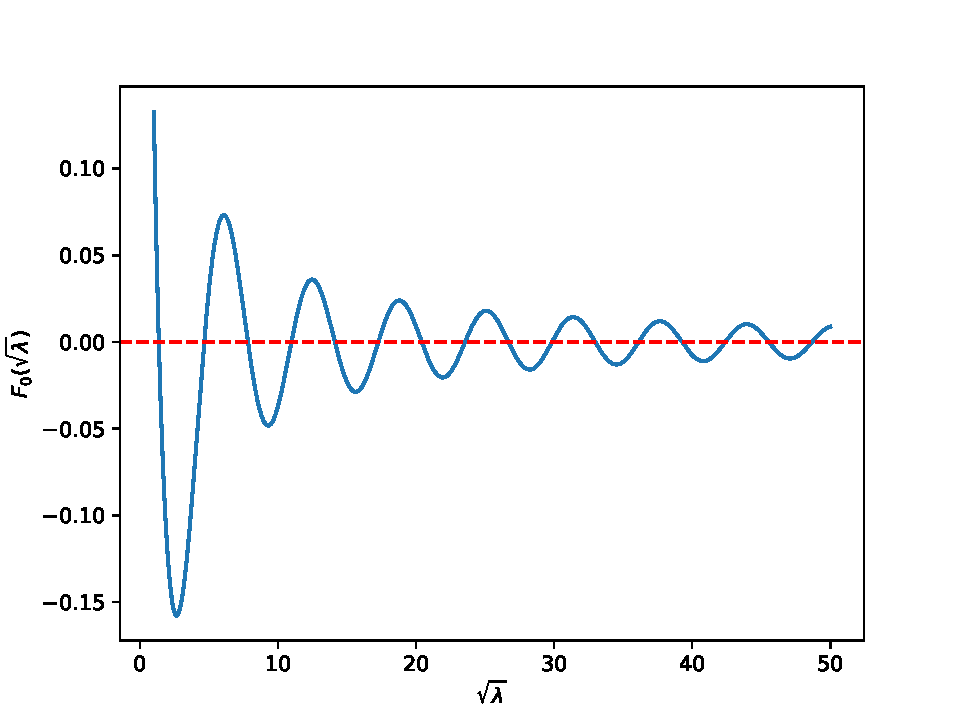
\includegraphics[width=0.5\textwidth]{F0}}%
  %\qquad
  \subfloat[]{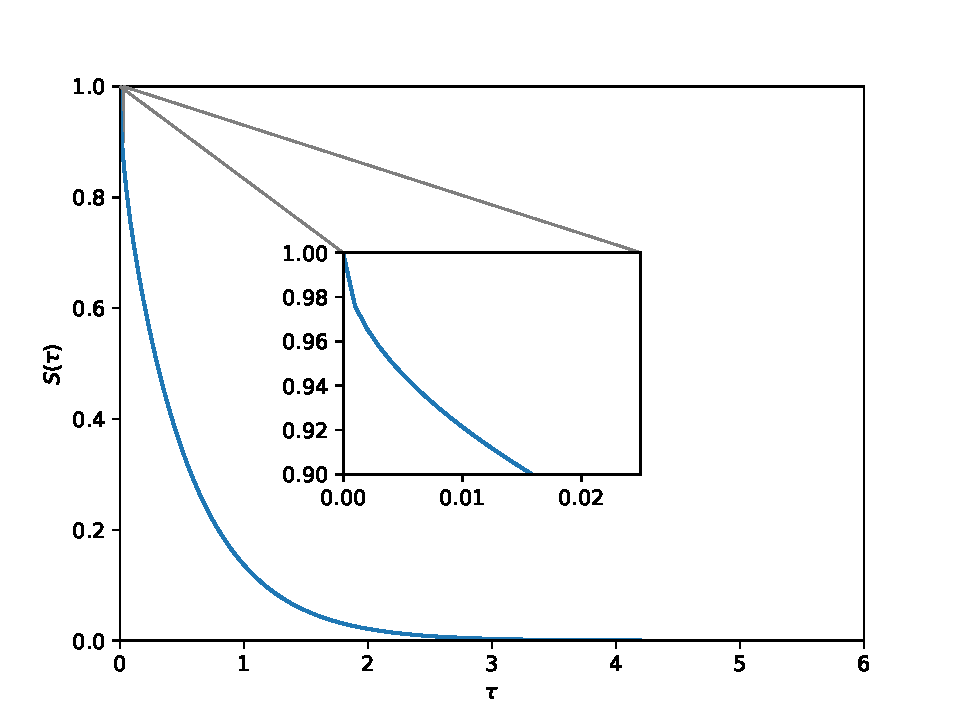
\includegraphics[width=0.5\textwidth]{analytical_s}}%
  \caption{(a) It is straightforward to evaluate the cross-product of
    Bessel fucntions by SciPy library \cite{2020SciPy-NMeth}. (b) The
    asymptotic behaviors of survival probability $S(\tau)$ are
    approximated by the numerical method with the first $1000$
    eigenvalues. $S(\tau)$ monotonously descrese from 1 at $\tau=0$ to
    $0$ as $\tau$ goes to infinity. Moreover, the approximation of
    analytical mean first-passage time $\langle \tau \rangle$ equals
    $0.47339248$.}
\end{figure}




